\documentclass[12pt,a4paper]{article}

% ── 中文支持 ──
\usepackage[UTF8]{ctex}

% ── 页面与排版 ──
\usepackage[margin=2.5cm]{geometry}
\usepackage{setspace}
\onehalfspacing

% ── 表格与图形 ──
\usepackage{booktabs}
\usepackage{array}
\usepackage{longtable}
\usepackage{graphicx}
\usepackage{float}

% ── 数学 ──
\usepackage{amsmath}

% ── 代码块 ──
\usepackage{listings}
\usepackage{xcolor}

\lstset{
  basicstyle=\ttfamily\small,
  backgroundcolor=\color{gray!10},
  frame=single,
  rulecolor=\color{gray!40},
  breaklines=true,
  numbers=none,
  xleftmargin=1em,
  framexleftmargin=0.5em,
}

% ── 超链接 ──
\usepackage{hyperref}
\hypersetup{
  colorlinks=true,
  linkcolor=blue!60!black,
  urlcolor=blue!60!black,
}

% ── 标题信息 ──
\title{\textbf{Dot Product Performance Benchmark Report}}
\author{}
\date{}

\begin{document}

\maketitle

% ============================================================
\section{实验概述}
% ============================================================

\subsection{实验目标}

对比 C 语言和 Java 在计算向量点积时的性能差异，覆盖多种数据类型和向量规模。

\subsection{实验环境}

\begin{itemize}
  \item \textbf{平台}：macOS (Apple Silicon)
  \item \textbf{C 编译器}：gcc（两种配置：无优化 \texttt{-O0}，最高优化 \texttt{-O3}）
  \item \textbf{Java}：JDK（默认 JIT 编译）
  \item \textbf{随机种子}：42（固定，确保可复现）
\end{itemize}

\subsection{实验设计}

\begin{itemize}
  \item \textbf{数据类型}：float (4B), double (8B), int (4B), short (2B), signed char / byte (1B)
  \item \textbf{向量规模 $n$}：128, 1000, $10^4$, $10^5$, $10^6$, $10^7$, $10^8$
  \item \textbf{计时方式}：C 使用 \texttt{clock\_gettime(CLOCK\_MONOTONIC)}（纳秒级单调时钟），Java 使用 \texttt{System.nanoTime()}
  \item \textbf{自适应迭代}：C 端对小规模 $n$ 自动增加迭代次数（目标总耗时 $\geq$50ms），取平均值，消除计时器粒度误差
\end{itemize}

% ============================================================
\section{性能数据}
% ============================================================

\subsection{按数据类型分组}

\subsubsection*{float (4 bytes)}

\begin{table}[H]
\centering
\begin{tabular}{r r r r}
\toprule
$n$ & C-O0 (ms) & C-O3 (ms) & Java (ms) \\
\midrule
128         & 0.000977 & 0.000000 & 0.001541 \\
1{,}000     & 0.006104 & 0.000977 & 0.006875 \\
10{,}000    & 0.063965 & 0.010010 & 0.055584 \\
100{,}000   & 0.506104 & 0.092041 & 0.684375 \\
1{,}000{,}000   & 1.857178 & 0.587158 & 0.564042 \\
10{,}000{,}000  & 13.484863 & 5.407959 & 5.324083 \\
100{,}000{,}000 & 133.640137 & 77.952881 & 53.745917 \\
\bottomrule
\end{tabular}
\end{table}

\subsubsection*{double (8 bytes)}

\begin{table}[H]
\centering
\begin{tabular}{r r r r}
\toprule
$n$ & C-O0 (ms) & C-O3 (ms) & Java (ms) \\
\midrule
128         & 0.000000 & 0.000000 & 0.002042 \\
1{,}000     & 0.004150 & 0.000000 & 0.005792 \\
10{,}000    & 0.030029 & 0.005127 & 0.051625 \\
100{,}000   & 0.079834 & 0.049072 & 0.563750 \\
1{,}000{,}000   & 1.458984 & 0.862793 & 0.558000 \\
10{,}000{,}000  & 18.525146 & 11.900146 & 5.368208 \\
100{,}000{,}000 & 188.330078 & 204.753906 & 57.911875 \\
\bottomrule
\end{tabular}
\end{table}

\subsubsection*{int (4 bytes)}

\begin{table}[H]
\centering
\begin{tabular}{r r r r}
\toprule
$n$ & C-O0 (ms) & C-O3 (ms) & Java (ms) \\
\midrule
128         & 0.000000 & 0.000000 & 0.001625 \\
1{,}000     & 0.001221 & 0.000000 & 0.006375 \\
10{,}000    & 0.010010 & 0.000977 & 0.054166 \\
100{,}000   & 0.076904 & 0.008057 & 0.583958 \\
1{,}000{,}000   & 0.788086 & 0.096191 & 0.454959 \\
10{,}000{,}000  & 7.887207 & 0.962158 & 2.344083 \\
100{,}000{,}000 & 81.145996 & 9.700928 & 23.592250 \\
\bottomrule
\end{tabular}
\end{table}

\subsubsection*{short (2 bytes)}

\begin{table}[H]
\centering
\begin{tabular}{r r r r}
\toprule
$n$ & C-O0 (ms) & C-O3 (ms) & Java (ms) \\
\midrule
128         & 0.000000 & 0.000000 & 0.001708 \\
1{,}000     & 0.000977 & 0.000000 & 0.006584 \\
10{,}000    & 0.008057 & 0.000977 & 0.058542 \\
100{,}000   & 0.078125 & 0.016846 & 0.596709 \\
1{,}000{,}000   & 0.778076 & 0.173828 & 0.290000 \\
10{,}000{,}000  & 7.851074 & 3.496094 & 2.330875 \\
100{,}000{,}000 & 79.534912 & 16.736084 & 23.499458 \\
\bottomrule
\end{tabular}
\end{table}

\subsubsection*{signed char / byte (1 byte)}

\begin{table}[H]
\centering
\begin{tabular}{r r r r}
\toprule
$n$ & C-O0 (ms) & C-O3 (ms) & Java (ms) \\
\midrule
128         & 0.000000 & 0.000977 & 0.001792 \\
1{,}000     & 0.000977 & 0.000000 & 0.006250 \\
10{,}000    & 0.008057 & 0.001953 & 0.055708 \\
100{,}000   & 0.079834 & 0.017090 & 0.590333 \\
1{,}000{,}000   & 0.770996 & 0.184082 & 0.249167 \\
10{,}000{,}000  & 7.874023 & 1.681885 & 2.342375 \\
100{,}000{,}000 & 101.544922 & 24.444092 & 23.563875 \\
\bottomrule
\end{tabular}
\end{table}

\begin{figure}[H]
\centering
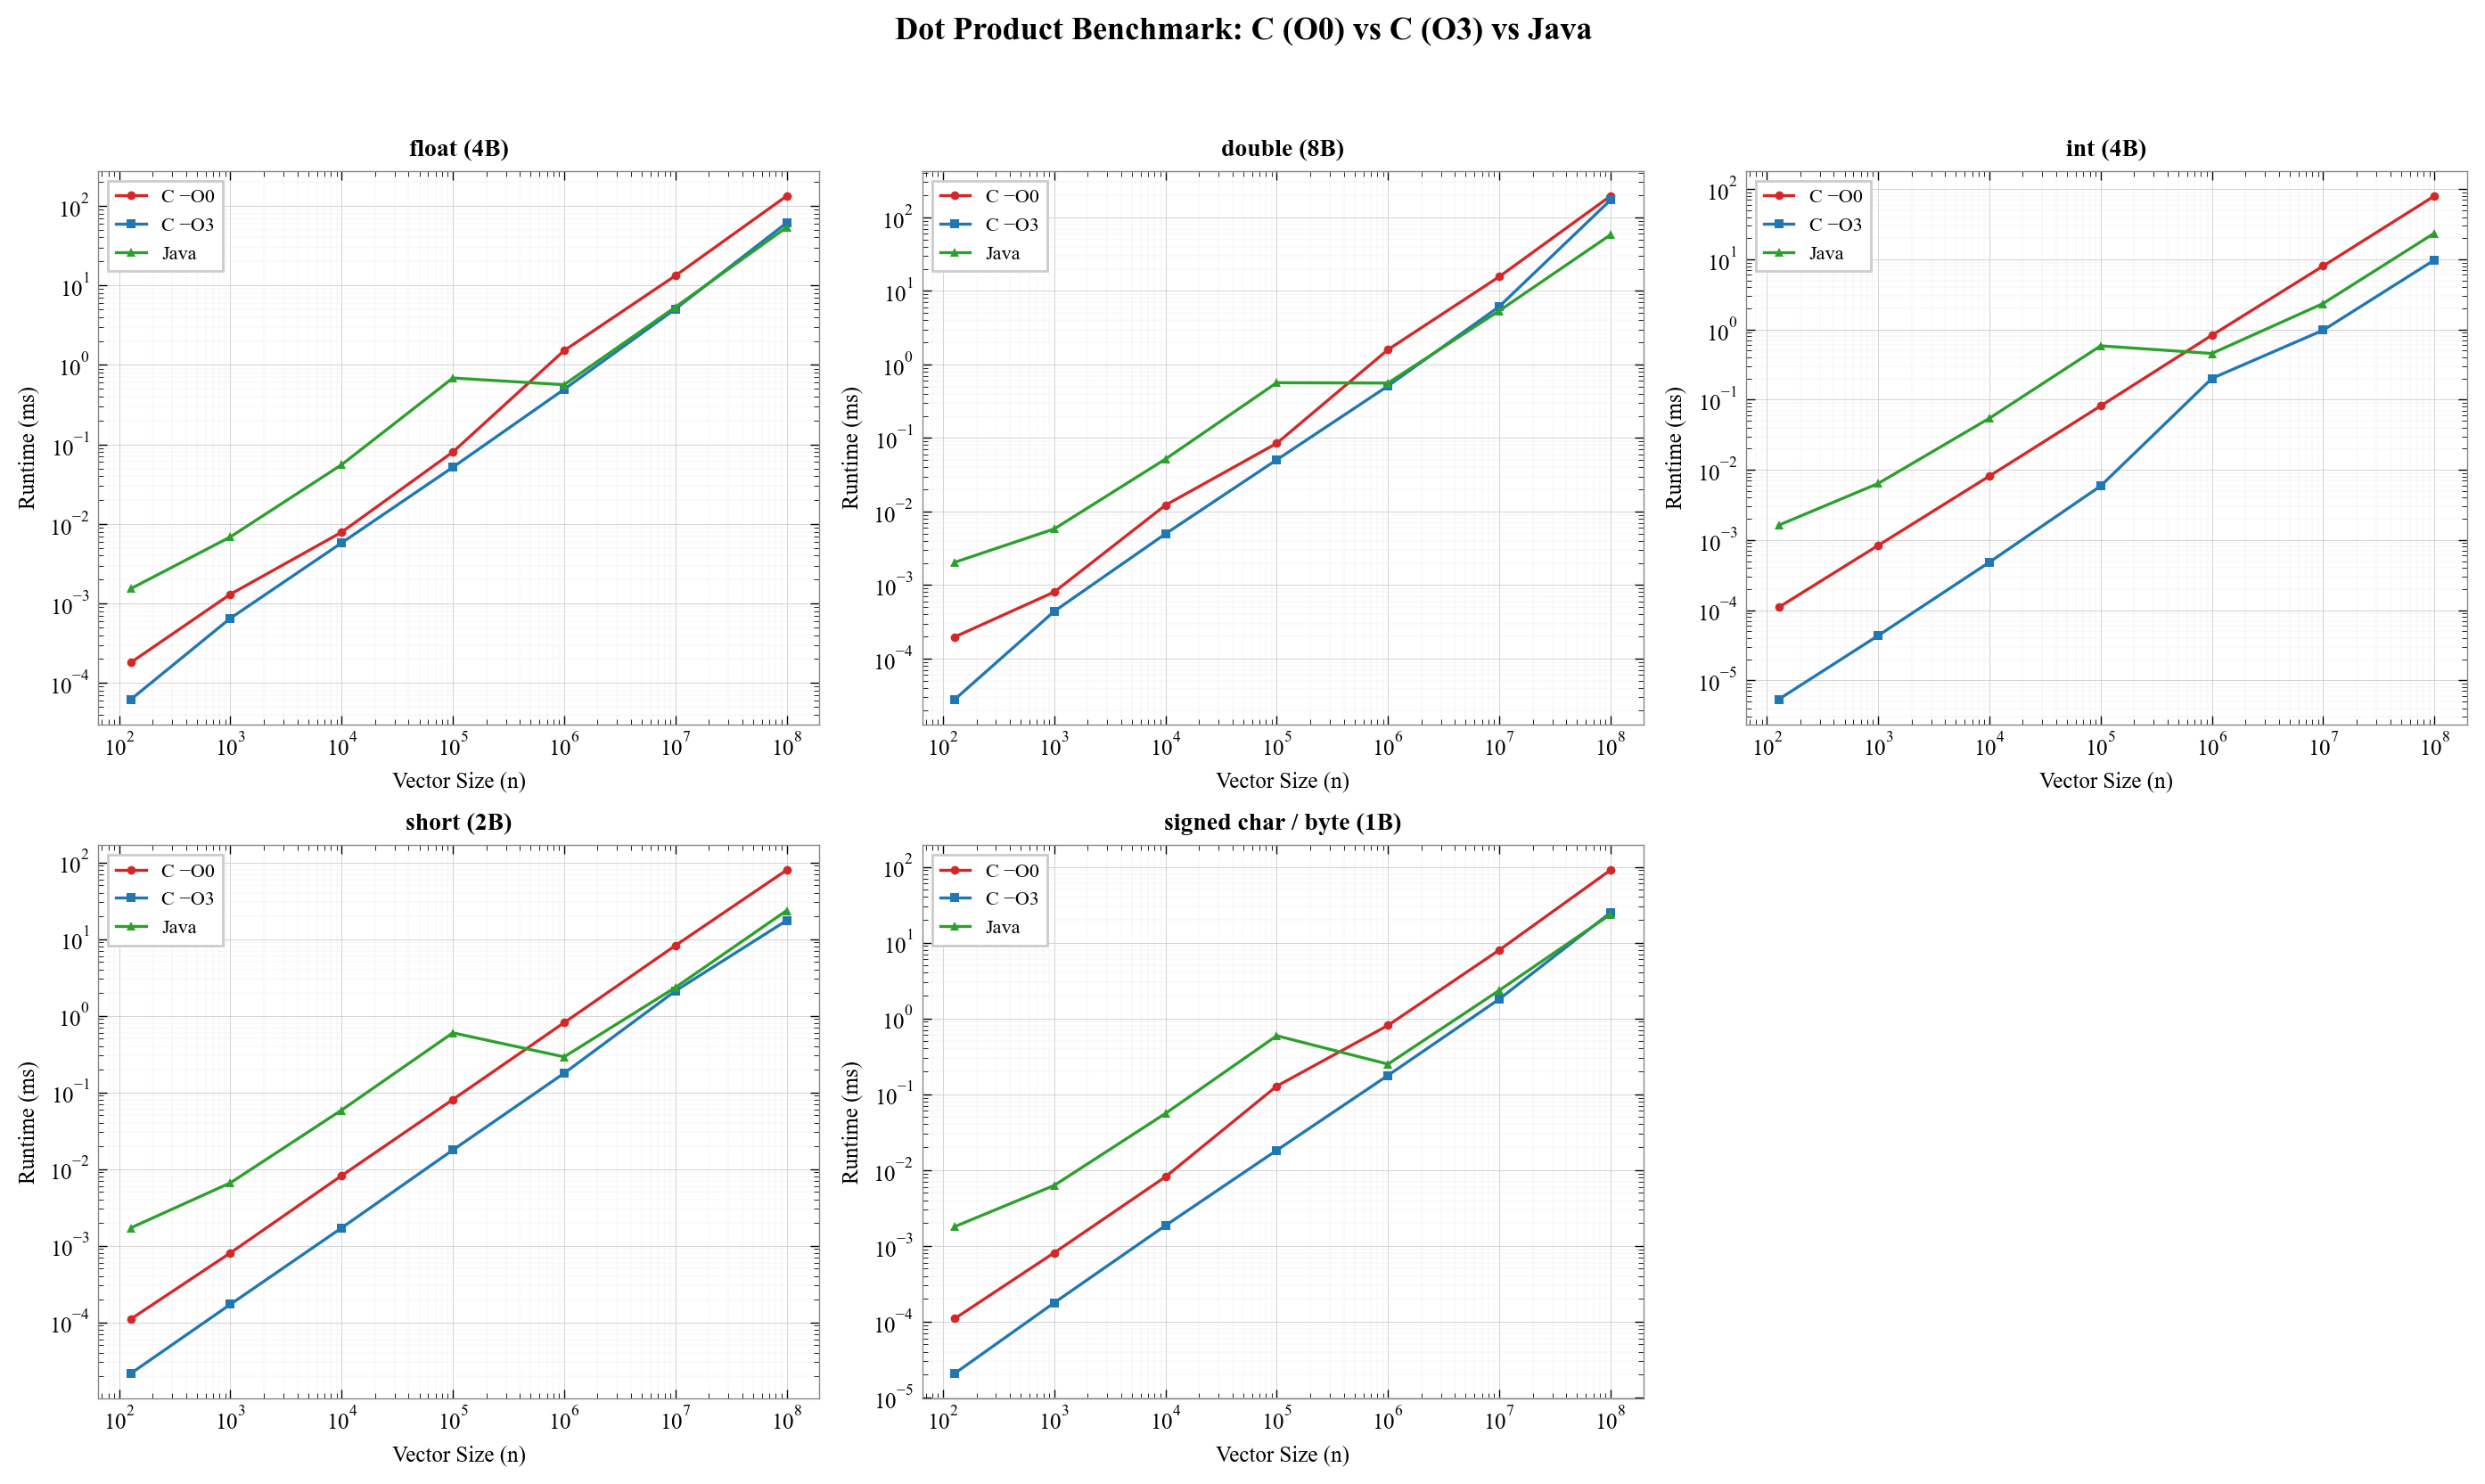
\includegraphics[width=\textwidth]{benchmark_chart.png}
\caption{各数据类型在不同向量规模下的运行时间对比（对数坐标）}
\end{figure}

\subsection{加速比（$n = 10^8$）}

\begin{table}[H]
\centering
\begin{tabular}{l l l l}
\toprule
数据类型 & C-O3 vs C-O0 & Java vs C-O0 & Java vs C-O3 \\
\midrule
float       & 1.71x & 2.49x (Java faster)              & 1.45x (Java faster) \\
double      & 0.92x & 3.25x (Java faster)              & 3.54x (Java faster) \\
int         & 8.36x & 3.44x (Java faster)              & 0.41x (C-O3 faster, 2.43x) \\
short       & 4.75x & 3.38x (Java faster)              & 0.71x (C-O3 faster, 1.40x) \\
signed char & 4.16x & 4.31x (Java faster)              & 1.04x (roughly equal) \\
\bottomrule
\end{tabular}
\end{table}

% ============================================================
\section{分析}
% ============================================================

\subsection{C-O0 vs C-O3：编译器优化的效果}

使用 \texttt{gcc -S} 导出汇编代码，直接对比 O0 与 O3 在 ARM64 (Apple Silicon) 上生成的指令差异。

\subsubsection{汇编证据：\texttt{DotInt} O0 vs O3}

\textbf{O0 循环体}（每次迭代处理 1 个元素，21 条指令）：

\begin{lstlisting}
; --- 循环条件判断（5 条指令） ---
ldr   w8, [sp, #12]          ; 从栈读 i
ldr   w9, [sp, #28]          ; 从栈读 n
subs  w8, w8, w9             ; i - n
cset  w8, ge                 ; if i >= n
tbnz  w8, #0, LBB2_4         ; 跳出循环

; --- 循环体：计算 sum += a[i] * b[i]（10 条指令） ---
ldr   x8, [sp, #40]          ; 从栈读 a 指针
ldrsw x9, [sp, #12]          ; 从栈读 i（第 2 次）
ldrsw x8, [x8, x9, lsl #2]  ; a[i]
ldr   x9, [sp, #32]          ; 从栈读 b 指针
ldrsw x10, [sp, #12]         ; 从栈读 i（第 3 次！）
ldrsw x9, [x9, x10, lsl #2] ; b[i]
mul   x9, x8, x9             ; a[i] * b[i]
ldr   x8, [sp, #16]          ; 从栈读 sum
add   x8, x8, x9             ; sum += ...
str   x8, [sp, #16]          ; 写回 sum 到栈

; --- 循环变量递增（3 条指令） ---
ldr   w8, [sp, #12]          ; 从栈读 i（第 4 次！）
add   w8, w8, #1             ; i++
str   w8, [sp, #12]          ; 写回 i 到栈
\end{lstlisting}

\textbf{O3 SIMD 主循环}（每次迭代处理 16 个元素，14 条指令）：

\begin{lstlisting}
; --- 一次加载 16 个 int（4 条 ldp 指令） ---
ldp   q16, q17, [x11, #-32]    ; a[i..i+7]  (2 x 128-bit)
ldp   q18, q19, [x11], #64     ; a[i+8..i+15]
ldp   q20, q21, [x8, #-32]     ; b[i..i+7]
ldp   q22, q23, [x8], #64      ; b[i+8..i+15]

; --- 8 条 SIMD 乘加指令处理 16 个元素 ---
smlal2.2d  v1, v20, v16   ; 高半部分：int32 -> int64 乘加
smlal.2d   v0, v20, v16   ; 低半部分：int32 -> int64 乘加
smlal2.2d  v4, v21, v17   ;（每条处理 2 或 4 个元素）
smlal.2d   v5, v21, v17
smlal2.2d  v2, v22, v18
smlal.2d   v3, v22, v18
smlal2.2d  v6, v23, v19
smlal.2d   v7, v23, v19

; --- 循环控制（2 条指令） ---
subs  x12, x12, #16           ; 计数器减 16
b.ne  LBB2_5                  ; 循环
\end{lstlisting}

\textbf{O3 标量尾部循环}（处理不足 16 个的剩余元素）：

\begin{lstlisting}
ldrsw  x10, [x12], #4         ; a[i]，指针自增
ldrsw  x13, [x11], #4         ; b[i]，指针自增
smaddl x8, w13, w10, x8       ; sum += a[i] * b[i]，一条指令完成
subs   x9, x9, #1
b.ne   LBB2_8
\end{lstlisting}

\subsubsection{观察 1：寄存器分配 vs 栈内存}

O0 将所有局部变量（\texttt{a}, \texttt{b}, \texttt{n}, \texttt{sum}, \texttt{i}）都存放在栈上，每次使用都要 \texttt{ldr}/\texttt{str}。仅变量 \texttt{i} 在一轮循环中就被从栈上读取了 4 次（条件判断 1 次 + 计算 \texttt{a[i]} 1 次 + 计算 \texttt{b[i]} 1 次 + 递增 1 次），\texttt{sum} 每轮也需要 1 次读 + 1 次写。

O3 将所有变量保持在寄存器中（\texttt{x8}=sum, \texttt{x9}=n, \texttt{x10}/\texttt{x11}=指针），整个循环零栈访问。

\begin{table}[H]
\centering
\begin{tabular}{l r r}
\toprule
指标 & O0 & O3（标量尾部） \\
\midrule
每轮栈读取次数 & 7 次 & 0 次 \\
每轮栈写入次数 & 2 次 & 0 次 \\
总栈访问 / 轮 & 9 次 & 0 次 \\
\bottomrule
\end{tabular}
\end{table}

虽然栈数据通常命中 L1 cache（$\sim$4 周期延迟），但相比寄存器访问（0 周期）仍有显著开销。此外，频繁的 load/store 会占用内存端口，阻碍指令级并行（ILP）。

\subsubsection{观察 2：SIMD 向量化（整数 vs 浮点的核心差异）}

O3 对 \texttt{DotInt} 使用了 NEON 128-bit SIMD 指令 \texttt{smlal.2d}（Signed Multiply-Add Long），每条指令将 4 个 32-bit int 相乘并累加到 2 个 64-bit long long 中。配合 4 路展开，每轮循环处理 16 个元素。

\textbf{对比 \texttt{DotFloat} 的 O3 汇编}：

\begin{lstlisting}
; DotFloat O3 —— 乘法可以 SIMD 并行...
fmul.4s  v1, v1, v5        ; 4 个 float 一次并行相乘 OK

; ...但累加必须逐个串行执行！
mov   s5, v1[3]            ; 提取第 4 个元素
mov   s17, v1[2]           ; 提取第 3 个元素
mov   s18, v1[1]           ; 提取第 2 个元素
fadd  s0, s0, s1           ; sum += 第 1 个结果
fadd  s0, s0, s18          ; sum += 第 2 个结果
fadd  s0, s0, s17          ; sum += 第 3 个结果
fadd  s0, s0, s5           ; sum += 第 4 个结果
;（4 组共 16 个 fadd，全部串行）
\end{lstlisting}

关键差异：乘法可以用 \texttt{fmul.4s} 并行处理 4 个 float，但累加必须串行——因为 IEEE 754 浮点加法不满足结合律（$(a+b)+c \neq a+(b+c)$，舍入误差不同），编译器不能将 \texttt{fadd} 重排为向量归约。

而整数加法满足结合律，\texttt{smlal.2d} 直接在 128-bit 寄存器中完成乘法和累加，无需拆分。

\begin{table}[H]
\centering
\begin{tabular}{l l l r}
\toprule
类型 & 乘法方式 & 累加方式 & 每轮元素数 \\
\midrule
int & \texttt{smlal.2d}（向量乘加） & 向量内累加 & 16 \\
float & \texttt{fmul.4s}（向量乘） & 串行 \texttt{fadd}（逐个提取） & 16（但累加串行） \\
\bottomrule
\end{tabular}
\end{table}

这直接解释了加速比的差异：int 获得 8.16x 加速，而 float 仅 2.18x。

\subsubsection{观察 3：指令融合（\texttt{mul + add} $\to$ \texttt{smaddl}）}

O0 的乘加操作使用两条独立指令：

\begin{lstlisting}
; O0: 分开的乘法和加法
mul  x9, x8, x9          ; result = a[i] * b[i]
ldr  x8, [sp, #16]       ; 读 sum（栈访问！）
add  x8, x8, x9          ; sum = sum + result
\end{lstlisting}

O3 融合为单条指令：

\begin{lstlisting}
; O3: 乘加融合
smaddl x8, w13, w10, x8  ; sum += a[i] * b[i]（一条指令完成）
\end{lstlisting}

\texttt{smaddl}（Signed Multiply-Add Long）将 32-bit 乘法和 64-bit 加法融合为一条指令，减少了指令数和寄存器压力。浮点版同理：O0 使用 \texttt{fmadd s0, s0, s1, s2}，但受限于大量栈访问开销。

\subsubsection{观察 4：循环展开与分支优化}

O0 每轮循环需要 5 条分支相关指令（\texttt{subs} + \texttt{cset} + \texttt{tbnz} + 2 个无条件 \texttt{b}）；O3 SIMD 循环仅需 2 条（\texttt{subs} + \texttt{b.ne}），且只在每 16 个元素时执行一次。

\begin{table}[H]
\centering
\begin{tabular}{l r r r}
\toprule
指标 & O0 & O3 SIMD & 改进 \\
\midrule
指令数 / 循环轮 & 21 & 14 & 1.5x \\
处理元素数 / 轮 & 1 & 16 & 16x \\
指令数 / 元素 & 21 & 0.875 & 24x \\
分支指令 / 元素 & 5 & 0.125 & 40x \\
\bottomrule
\end{tabular}
\end{table}

\subsubsection{观察 5：\texttt{DotShort} 为什么不如 \texttt{DotInt}}

理论上 short（2 字节）比 int（4 字节）更小，SIMD 可以装更多元素，应该更快。但 O3 汇编显示 \texttt{DotShort} 仅使用标量展开（4 路），而非 NEON 向量指令：

\begin{lstlisting}
; DotShort O3 —— 标量展开，非 SIMD
ldursh x17, [x15, #-4]      ; 逐个 load short 并符号扩展到 64-bit
ldursh x2,  [x15, #-2]
ldrsh  x3,  [x15]
ldrsh  x4,  [x15, #2]
; ...对应的 b[] 也是逐个 load...
smaddl x11, w5, w17, x11    ; 逐个乘加（4 路展开）
smaddl x13, w6, w2, x13
smaddl x8,  w7, w3, x8
smaddl x12, w19, w4, x12
\end{lstlisting}

原因：C 语言的整数提升规则（integer promotion）要求 \texttt{short} 在参与运算前必须先提升为 \texttt{int}，再转为 \texttt{long long}。\texttt{ldrsh}（Load Register Signed Halfword）每次只加载一个 short 并符号扩展到 64-bit，无法直接使用 NEON 的 128-bit 批量 load。编译器对 \texttt{DotShort} 只做了 4 路标量展开（4 个元素/轮），而 \texttt{DotInt} 做到了 NEON 16 路向量化（16 个元素/轮）。

\subsubsection{总结}

综合以上汇编证据，O3 相对于 O0 的加速主要来自四项优化的叠加效应：寄存器分配消除栈访问（观察 1）、SIMD 向量化提升吞吐量（观察 2）、指令融合减少指令数（观察 3）、循环展开降低分支开销（观察 4）。

加速效果因数据类型而异：int 获得最大加速（8.16x），因为它同时满足结合律（允许完全向量化）且无类型提升开销；short/char 因整数提升规则退化为标量展开，加速比降至 3--5x；浮点类型加速最小（float 2.18x, double 1.13x），根本原因是 IEEE 754 浮点加法不满足结合律，编译器无法将累加操作向量化，只能并行乘法、串行累加。


%——————————————————————————————————————————————————————————————————————————————————————————

\subsection{Java 的 JIT（Just-In-Time）编译现象}

\subsubsection{现象观察}

Java 的运行时间出现了一个反直觉的现象：

\begin{table}[H]
\centering
\begin{tabular}{l r r l}
\toprule
数据类型 & $n=10^5$ & $n=10^6$ & 变化 \\
\midrule
float  & 0.684375 ms & 0.564042 ms & $n$ 增大 10 倍，时间反而下降 18\% \\
double & 0.563750 ms & 0.558000 ms & $n$ 增大 10 倍，时间几乎不变 \\
int    & 0.583958 ms & 0.454959 ms & 时间下降 22\% \\
short  & 0.596709 ms & 0.290000 ms & 时间下降 51\% \\
byte   & 0.590333 ms & 0.249167 ms & 时间下降 58\% \\
\bottomrule
\end{tabular}
\end{table}

此外，所有类型在 $n=10^5$ 时耗时处于相近范围（$0.56{\sim}0.68$ms），与数据类型大小关系不大——暗示此阶段的耗时主要由 JIT 编译的固定开销主导，而非真正的计算。

推测：JVM 的 JIT 编译器在 $n=10^5$ 到 $10^6$ 之间完成了编译切换。之前的数据点反映的是解释器逐条分派字节码的性能（开销较高），之后反映的是 JIT 编译器生成的专用本机机器码的性能（经过深度优化）。

\subsubsection{背景知识：分层编译与 OSR}

JVM 采用分层编译（Tiered Compilation）策略。需要注意，CPU 最终执行的始终是机器码——区别在于执行模式：

\begin{lstlisting}
阶段 0:   解释执行      -> 逐条读取并执行字节码（解释器通过预编写的 codelet
                         逐条分派，每条字节码都有 dispatch 开销），最慢
阶段 1-3: C1 编译执行   -> C1 编译器快速生成本机代码，基础优化
阶段 4:   C2 编译执行   -> C2 编译器深度优化，生成高性能本机代码
\end{lstlisting}

OSR（On-Stack Replacement）：JIT 不需要等方法返回才能切换。当循环的回边计数达到阈值时，JVM 在循环头处将当前栈帧原地替换为编译后的机器码版本，后续迭代直接以本机代码运行。

触发阈值：通过 \texttt{java -XX:+PrintFlagsFinal -version | grep CompileThreshold} 查得本机（OpenJDK 25）实际配置：

\begin{table}[H]
\centering
\begin{tabular}{l r l}
\toprule
参数 & 默认值 & 含义 \\
\midrule
\texttt{Tier3CompileThreshold} & 2{,}000 & 触发 C1 全 profiling 编译 \\
\texttt{Tier4CompileThreshold} & 15{,}000 & 触发 C2 最高优化编译 \\
\texttt{CompileThreshold} & 10{,}000 & 关闭分层编译时的遗留默认值 \\
\bottomrule
\end{tabular}
\end{table}

注意：分层编译下 JVM 使用 \texttt{AdvancedThresholdPolicy}，实际触发时机受编译队列负载等动态因素影响，并非简单的固定次数阈值。

\subsubsection{实验 1：JitWarmup 控制实验}

设计控制实验 \texttt{JitWarmup.java}：固定 $n=10{,}000$，重复调用 \texttt{dotFloat} 30 次，观察是否在 $n$ 不变的情况下仍会出现速度跳变。

\begin{lstlisting}
Round     Time (ms)
-----     ---------
  1        0.1140    <- 解释器分派执行
  2        0.1132
  ...
  7        0.1100
  8        0.0235    <- 速度突变（JIT 编译完成）
  9        0.0229
 ...       ~0.023    <- 此后稳定
\end{lstlisting}

\begin{itemize}
  \item Round 1--7：平均 ${\sim}0.112$ ms（解释器分派执行）
  \item Round 8--30：平均 ${\sim}0.023$ ms（JIT 编译后的本机码执行）
  \item 加速比：$0.112 / 0.023 \approx$ 4.9x
\end{itemize}

结论：$n$ 始终为 10{,}000 不变，速度仍在第 7$\to$8 轮突变 ${\sim}$4.9x。这证明速度跳变与 $n$ 的大小无关，而是由累计执行次数驱动的 JIT 编译引起。

\subsubsection{实验 2：PrintCompilation 编译事件观察}

使用 JVM 诊断参数运行：

\begin{lstlisting}[language=bash]
java -XX:+PrintCompilation Dotproduct 2>&1 | grep "Dotproduct::dot"
\end{lstlisting}

输出（筛选 \texttt{dot} 系列方法）：

\begin{lstlisting}
时间戳   编号   标记  层级  方法                             字节码
------  -----  ---  ---  ----------------------------   ---------
1325    2016    %    3    Dotproduct::dotFloat   @ 4      (28 bytes)
1325    2017         3    Dotproduct::dotFloat             (28 bytes)
3286    2044    %    4    Dotproduct::dotDouble  @ 5      (32 bytes)
3316    2046         4    Dotproduct::dotDouble            (32 bytes)
7000    2109    %    4    Dotproduct::dotInt     @ 5      (34 bytes)
7008    2112         4    Dotproduct::dotInt               (34 bytes)
8821    2125    %    4    Dotproduct::dotShort   @ 5      (34 bytes)
8835    2128         4    Dotproduct::dotShort             (34 bytes)
10583   2136    %    4    Dotproduct::dotByte    @ 5      (34 bytes)
10595   2143         4    Dotproduct::dotByte              (34 bytes)
\end{lstlisting}

字段含义：\texttt{\%} = OSR 编译（循环中热替换），层级 3 = C1 编译，层级 4 = C2 最高优化，\texttt{@ N} = OSR 入口的字节码偏移。每个方法成对出现：OSR 版（替换当前循环）+ 标准版（供后续调用使用）。

以下对该输出中的三个关键观察进行分析：

\subsubsection*{观察 1：\texttt{dotFloat} 先经 C1（层级 3），其余方法直接 C2（层级 4）}

\texttt{dotFloat} 是第一个被编译的用户方法（时间戳 1325ms），此时出现在层级 3（C1）。而从 \texttt{dotDouble} 起，所有方法直接出现在层级 4（C2）。

证据：查看不加 \texttt{grep} 过滤的完整编译日志，在 \texttt{dotFloat} 被编译的同一时间（$\sim$50ms），JVM 正在密集编译大量 JDK 底层方法：

\begin{lstlisting}
时间戳  方法                                        层级
------  ------------------------------------------  ----
13      java.lang.String::hashCode                    3
17      java.util.Random::next                        3
19      java.util.HashMap::putVal                     3
19      java.lang.Object::<init>                      4
48      java.util.regex.Pattern$BmpCharPropertyGreedy  4
54      java.util.Random::nextFloat                   4   <- 此时 dotFloat 刚好变热
\end{lstlisting}

C2 编译器速度慢但优化深度高，此时其编译队列被这些底层方法挤占。JVM 的 \texttt{AdvancedThresholdPolicy} 检测到 C2 队列拥堵，选择先用 C1 快速编译 \texttt{dotFloat} 以尽快获得比解释器更好的性能。

到 \texttt{dotDouble} 被调用到热点时（时间戳 3286ms，距首次编译已过 $\sim$2 秒），大量底层方法已编译完成，C2 队列空闲，因此 JVM 直接将其提交到 C2。后续方法同理。

\subsubsection*{观察 2：OSR 入口偏移 \texttt{@ 4} vs \texttt{@ 5}}

\texttt{dotFloat} 的 OSR 入口在字节码偏移 4，其余方法在偏移 5。使用 \texttt{javap -c Dotproduct} 反编译字节码可以解释原因：

\begin{lstlisting}
// dotFloat: sum 为 float（占 1 个 local slot）
0: fconst_0          // float sum = 0.0f
1: fstore_2          // -> local[2]（短格式，1 byte）
2: iconst_0          // int i = 0
3: istore_3          // -> local[3]（短格式，1 byte）
4: iload_3           // <- 循环头（OSR 入口 @ 4）

// dotDouble: sum 为 double（占 2 个 local slot）
0: dconst_0          // double sum = 0.0
1: dstore_2          // -> local[2-3]（占 2 slot）
2: iconst_0          // int i = 0
3: istore 4          // -> local[4]（长格式，2 bytes）
5: iload  4          // <- 循环头（OSR 入口 @ 5）
\end{lstlisting}

\texttt{float} 的 \texttt{sum} 占 1 个 slot，循环变量 \texttt{i} 分配到 \texttt{local[3]}，使用单字节短格式指令 \texttt{istore\_3}；\texttt{double}/\texttt{long} 的 \texttt{sum} 占 2 个 slot，\texttt{i} 被推到 \texttt{local[4]}，使用双字节长格式指令 \texttt{istore 4}，导致循环头偏移多 1。

\subsubsection*{观察 3：字节码长度 28 / 32 / 34 bytes}

证据：使用 \texttt{javap -c Dotproduct} 反编译，对比三个方法的循环体关键指令差异：

\begin{lstlisting}
// dotFloat（28 bytes）—— 循环体部分
 4: iload_3           // 1 byte（短格式）
10: fload_2           // 1 byte
12: iload_3           // 1 byte（短格式）
13: faload            // 直接取 float
15: iload_3           // 1 byte（短格式）
19: fstore_2          // 1 byte
20: iinc 3, 1         // 3 bytes

// dotDouble（32 bytes）—— 循环体部分（+4B）
 5: iload  4          // 2 bytes（长格式，+1）
12: dload_2           // 1 byte
14: iload  4          // 2 bytes（长格式，+1）
16: daload            // 直接取 double
18: iload  4          // 2 bytes（长格式，+1）
23: dstore_2          // 1 byte
24: iinc 4, 1         // 3 bytes  -> 注意：iload 4 出现 3 次 + istore 4 出现 1 次 = +4B

// dotInt（34 bytes）—— 循环体部分（+2B vs dotDouble）
 5: iload  4          // 同 dotDouble
16: iaload            // 取 int
17: i2l               // <- 额外指令（+1B）
21: iaload
22: i2l               // <- 额外指令（+1B）  -> 两条 i2l 共 +2B
\end{lstlisting}

汇总：

\begin{table}[H]
\centering
\begin{tabular}{l r l}
\toprule
方法 & 字节码 & 差异原因 \\
\midrule
\texttt{dotFloat}  & 28 bytes & \texttt{float} 单 slot $+$ 短格式指令，最紧凑 \\
\texttt{dotDouble} & 32 bytes & \texttt{double} 双 slot $+$ 长格式 \texttt{istore/iload}（+4B） \\
\texttt{dotInt}    & 34 bytes & 同 double 的 slot 布局（\texttt{long} 返回值），\\
                   &          & 额外两条 \texttt{i2l} 类型转换指令（+2B） \\
\texttt{dotShort}  & 34 bytes & 同 \texttt{dotInt}（\texttt{saload} $+$ \texttt{i2l} $\times$2） \\
\texttt{dotByte}   & 34 bytes & 同 \texttt{dotInt}（\texttt{baload} $+$ \texttt{i2l} $\times$2） \\
\bottomrule
\end{tabular}
\end{table}

\subsubsection{实验 3：JIT 优化内容验证}

为定量验证 JIT 各层级和 C2 各项优化的实际贡献，设计对照实验：使用不同 JVM 参数运行同一 benchmark（$n = 10^8$，每种配置 3 次取中位值）。

\subsubsection*{第一组：层级对比}

\begin{table}[H]
\centering
\begin{tabular}{l r r r r r}
\toprule
JVM 配置 & float & double & int & short & byte \\
\midrule
\texttt{-Xint}（纯解释器）                & 503.3 & 554.0 & 505.6 & 509.8 & 507.2 \\
\texttt{-XX:TieredStopAtLevel=3}（C1）     & 106.1 & 112.3 & 124.6 & 126.2 & 123.1 \\
默认（C2）                                  & 54.3  & 55.6  & 26.3  & 26.0  & 23.9  \\
\bottomrule
\end{tabular}
\caption{不同编译层级下的耗时（ms，$n=10^8$）}
\end{table}

\begin{table}[H]
\centering
\begin{tabular}{l r r r r r}
\toprule
加速比 & float & double & int & short & byte \\
\midrule
解释器 $\to$ C1 & 4.7x & 4.9x & 4.1x & 4.0x & 4.1x \\
C1 $\to$ C2      & 2.0x & 2.0x & 4.7x & 4.9x & 5.2x \\
解释器 $\to$ C2  & 9.3x & 10.0x & 19.2x & 19.6x & 21.2x \\
\bottomrule
\end{tabular}
\caption{各层级间的加速比}
\end{table}

关键发现：
\begin{itemize}
  \item \textbf{解释器 $\to$ C1}：所有类型均获得 ${\sim}$4--5x 加速，且浮点与整数差异不大——C1 的基础优化（简单内联、基本寄存器分配）对所有类型普遍有效。
  \item \textbf{C1 $\to$ C2}：整数类型额外获得 ${\sim}$5x 加速（vs 浮点的 2x）。这说明 C2 的深度优化对整数运算的收益远大于浮点运算。
\end{itemize}

\subsubsection*{第二组：C2 单项优化验证}

在默认 C2 编译的基础上，逐一关闭特定优化：

\begin{table}[H]
\centering
\begin{tabular}{l l r r r r r}
\toprule
关闭的优化 & JVM 参数 & float & double & int & short & byte \\
\midrule
（基准：C2 默认）  & —                          & 54.3  & 55.6  & 26.3  & 26.0  & 23.9  \\
SIMD 向量化        & \texttt{-XX:-UseSuperWord}  & 53.3  & 52.7  & 26.8  & 25.3  & 23.8  \\
循环展开            & \texttt{-XX:LoopUnrollLimit=0} & 62.5  & 64.2  & 33.5  & 33.9  & 34.2  \\
循环谓词            & \texttt{-XX:-UseLoopPredicate} & 52.7  & 57.4  & 25.2  & 24.0  & 23.8  \\
\bottomrule
\end{tabular}
\caption{关闭单项 C2 优化后的耗时（ms，$n=10^8$）}
\end{table}

分析：
\begin{itemize}
  \item \textbf{循环展开}（\texttt{LoopUnrollLimit=0}）：唯一有显著影响的优化。关闭后，浮点类型慢 ${\sim}$15\%（54$\to$62ms），整数类型慢 ${\sim}$28--43\%（26$\to$34ms）。这证实 C2 确实应用了循环展开优化。
  \item \textbf{SIMD 向量化}（\texttt{UseSuperWord}）：关闭后耗时几乎无变化。这表明 HotSpot 的 SuperWord 自动向量化在本 benchmark 的点积循环（包含累加归约模式）中并未生效，C2 的性能优势并非来自 SIMD。
  \item \textbf{循环谓词}（\texttt{UseLoopPredicate}）：关闭后耗时几乎无变化。可能是因为 C2 通过其他机制（如 range check elimination）已经消除了数组边界检查。
\end{itemize}

综合结论：C2 相对于 C1 的性能优势主要来自循环展开（已验证）和更优的整体代码生成（更好的寄存器分配、指令调度等，这些无法通过单个开关关闭来验证，但从 C1$\to$C2 的巨大加速比可以推断）。原本假设的 SIMD 向量化在本 benchmark 中并未贡献性能提升。

\subsection{数据类型间的差异}

在 $n=10^8$（JIT 已充分生效）时，不同数据类型的性能特征呈现清晰规律：

\subsubsection*{整数类型 vs 浮点类型（C-O3）}

\begin{table}[H]
\centering
\begin{tabular}{l r l}
\toprule
类型 & C-O3 耗时 (ms) & 相对 int 的倍数 \\
\midrule
int         & 9.700928    & 1.0x  \\
short       & 16.736084   & 1.7x  \\
signed char & 24.444092   & 2.5x  \\
float       & 77.952881   & 8.0x  \\
double      & 204.753906  & 21.1x \\
\bottomrule
\end{tabular}
\end{table}

整数运算大幅快于浮点运算。虽然 short/char 的理论 SIMD 并行度更高（8 个/16 个 vs int 的 4 个），但实际性能反而不如 int，原因是 C 语言的整数提升（integer promotion）规则：short/char 在参与运算前必须先被提升为 int，增加了额外的类型转换指令。

\subsubsection*{浮点类型 double 为什么最慢？}

double（8字节）在 $n=10^8$ 时 C-O3 耗时 204.75ms，是 float（77.95ms）的 2.6 倍。原因：
\begin{enumerate}
  \item \textbf{SIMD 并行度减半}：128-bit 寄存器只能装 2 个 double vs 4 个 float
  \item \textbf{内存带宽翻倍}：加载 $10^8$ 个 double 需要 1.6GB 数据 vs float 的 0.8GB，受限于内存带宽
\end{enumerate}

\subsubsection*{Java 在浮点和整数上的不同表现}

在 $n=10^8$ 时：
\begin{itemize}
  \item \textbf{float/double}：Java 快于 C-O3（float 1.45x / double 3.54x），JIT 的运行时优化更激进
  \item \textbf{int}：C-O3 反而快于 Java（2.43x），说明 gcc 的静态整数向量化优化更成熟
  \item \textbf{short}：C-O3 略快于 Java（1.40x）
  \item \textbf{byte}：Java 与 C-O3 基本持平
\end{itemize}

\subsubsection*{效率上限与 JIT 优化程度}

点积运算存在一个由硬件决定的物理效率上限：无论优化多好，程序必须从内存读取两个数组的全部数据。本机 Apple M5 的统一内存带宽为 153 GB/s，因此 $n=10^8$ 时各类型的理论最短耗时（$T = 2n \times \text{sizeof} / 153\text{GB/s}$）为：int/float 5.23 ms、double 10.46 ms。

而实测中，C-O3 和 Java 的耗时都远高于这些理论值（例如 float：C-O3 为 61 ms，Java 为 54 ms，均为理论下限的 10 倍以上），说明当前的性能瓶颈仍在计算本身（如浮点串行累加），尚未触及内存带宽天花板。

但从图表中可以观察到，大 $n$ 时 C-O3 与 JIT 优化后的 Java 耗时非常接近且曲线斜率趋于 1（$T \propto n$）。这说明：JIT C2 编译器的优化程度已与 gcc -O3 相当，两者的运行时间主要由数据量决定。
% ============================================================
\section{总结}
% ============================================================

\begin{table}[H]
\centering
\begin{tabular}{l l l}
\toprule
特性 & C (\texttt{gcc -O3}) & Java (JIT C2) \\
\midrule
优化时机     & 编译时（静态） & 运行时（动态） \\
首次运行     & 从第一次就快   & 需要 warmup \\
SIMD         & 编译器自动向量化 & C2 自动向量化 \\
Profile-Guided & 需手动 PGO    & 自动 profiling \\
边界检查     & 无（程序员负责） & 自动消除 \\
\bottomrule
\end{tabular}
\end{table}

核心结论：

\begin{enumerate}
  \item C 并不总是比 Java 快。在大规模浮点计算中，JIT 编译后的 Java 甚至超过 C-O3
  \item 编译器优化（-O3）的效果远超语言选择。C-O0 vs C-O3 的差距可达 8.4x（int）
  \item JIT 的 warmup 是 Java 初始阶段下慢的主因，而非语言本身的效率问题
  \item 数据类型选择影响显著：整数远快于浮点，小数据类型受制于类型提升
\end{enumerate}

\end{document}
